\subsection{AST-Generation}
\label{chap:ast_generation}

Even though the CST already contains all relevant information about the sources, 
it is very verbose, and the structure of the CST is usually not very friendly to work with.
For this reason, \verb|gp-modifiable-ast| implements the modifiers provided by \cite{GeneratingRewritableAST}, 
which are used to convert the CST into an AST.

There are three types of nodes in the AST. \verb|ProductionTreeNode| are nodes derived from a grammar production. 
\verb|TokenTreeNode| are nodes derived from a lexer token. 
\verb|StringTreeNode| are nodes that contain a string and are used to replace other tree nodes. 
The \verb|StringTreeNode| is not part of the initial AST. 
This node can be used by the user to replace subtrees in the final AST or to add a new node.
 
Any \verb|TokenTreeNode| that references a token from \verb|HIDDEN_LEXER_RULES| is marked as hidden. 
These nodes are stored in the AST, but are not visible to the user unless specifically requested. 
Next, the AST structure is modified by the modifiers defined in the grammar file. 
Each modifier has its own implementation and is applied bottom-up for each node.

\subsubsection{list-Modifier}

The \verb|list| modifier, proposed by \cite{GeneratingRewritableAST}, is a modifier designed to flatten out self-recursive productions. 
This modifier can only be applied to symbols on the left side of a production. 
The following example could be a production for the function parameters in common programming languages.

\begin{lstlisting}[caption=list modifier example]
PARAMETER_LIST[list] -> PARAMETER_LIST PARAMETER | 
                        PARAMETER | 
                        EPSILON;
\end{lstlisting}

This grammar rule generates the following CST for an input with for example three parameters.


\begin{figure}[H]
    \centering
    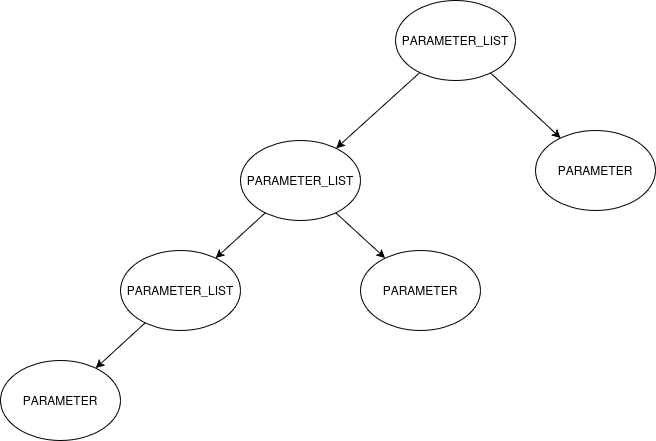
\includegraphics[scale=0.4]{"fig/list_modifier_cst.png"}
    \caption{CST before the list modifier is applied}
\end{figure}

This structure is too verbose and difficult to work with in practice, so by using the \verb|[list]| modifier, we get the following AST.

\begin{figure}[H]
    \centering
    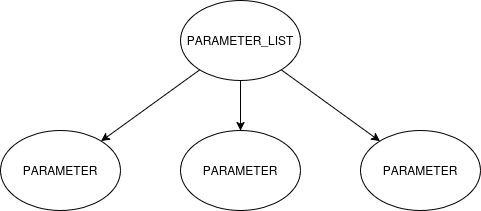
\includegraphics[scale=0.4]{"fig/list_modifier_ast.png"}
    \caption{AST after the list modifier is applied}
\end{figure}

This structure is much easier to manage and still contains all relevant information about the sources.

The modifier is applied by checking if the children of the current \verb|ProductionTreeNode| $n$ contain a \verb|ProductionTreeNode| $m$ that references the same production. If so, $m$ is replaced in the children list of $n$ by all children of $m$.
Since the modifiers are applied bottom-up, this works for nested trees.

\subsubsection{alias-Modifier}

The \verb|alias| modifier, proposed by  \cite{GeneratingRewritableAST}, is a modifier that can be applied to any symbol on the right hand side of a production. 
This modifier, adds an alias to the tree node that can be used to search the tree. 
The following could be an example of a production for addition in a programming language.

\begin{verbatim}
ADD -> NUMBER[alias=left] plus NUMBER[alias=right];
\end{verbatim}

Without the alias modifier, the only way to distinguish between the two \verb|NUMBER| nodes would be by the order of the children of the \verb|ADD| tree node. 
The \verb|alias| modifier allows for cleaner searches in the AST.

This modifier is applied by simply storing the alias in the tree node.


\subsubsection{hidden-Modifier}

The \verb|hidden| modifier, proposed by \cite{GeneratingRewritableAST}, is a modifier that can be applied to terminal symbols on the right hand side of a production.
This modifier will hide the tree node in the AST. 
In the previous example of the \verb|ADD| production, the \verb|ADD| tree node would have a \verb|TokenTreeNode| child that references the \verb|plus| lexer definition. 
This information is obsolete because the production will always contain this node, and the production name already contains the necessary information. 
By applying the \verb|hidden| modifier to the \verb|plus| symbol, the corresponding tree node will still exist, but will not be visible unless specifically requested.

\subsubsection{inline-Modifier}

The \verb|inline| modifier, proposed by \cite{GeneratingRewritableAST}, is a modifier that can be applied to nonterminal symbols on the right hand side of a production. 

Applying the modifier will replace the node with all its children. 
This modifier should be used on nonterminals that do not carry important information themselves, but their children do. 
This way all information is preserved, but the tree structure is simplified.

The following grammar should illustrate the purpose of this modifier.

\begin{lstlisting}[caption=inline modifier example grammar]
EXPRESSION              ->      ARITHMETIC_EXPRESSION[inline];
ARITHMETIC_EXPRESSION   ->      PLUS_EXPRESSION;
PLUS_EXPRESSION         ->      integer plus integer;
\end{lstlisting}

The \lstinline{ARITHMETIC_EXPRESSION} production is only used for creating the grammar in this case, as it may not be possible to create an LR(1) grammar without it.
Another reason for defining a grammar this way is to prevent duplications. If \lstinline{ARITHMETIC_EXPRESSION} is also used at other places in the grammar file,
the extraction into a new production can reduce the total size of a grammar definition and improve the maintainability.

This production carries however no information itself that are relevant to the program structure, therefore it can be ommitted in the AST.

This modifier is implemented by replacing all \verb|ProductionTreeNodes| that have this modifier with their corresponding children.

Therefore, the resulting AST does not contain the \lstinline{ARITHMETIC_EXPRESSION} node.

\subsubsection{Not implemented modifiers}

\cite{GeneratingRewritableAST} proposed additional modifiers that are not implemented in \verb|gp-modifiable-ast|.
The first is the \verb|Boolean Access| modifier, which would replace a node with a boolean value depending on whether that symbol was parsed. 
However, since we do not generate classes for every production, this would be of little use.
The same reason applies to the \verb|superclass| modifier, which would create a hierarchy in the generated classes of the parser generator.
